\section*{REGRESSION}\label{regression}
The ship power data is split into a train and a test part. In the time
series the samples are not independent, which means that splitting the
data into a train and test set should not be done randomly! With a time
series, training should be done on historic data to predict the future.
This means that the training set must happen in time prior to the test
set. Fig.\ref{fig:train_test} shows how the train-test-split
should been done for the present data, where the last 20\% of the data
is used for testing.
In Fig.\ref{fig:test_size_variation} this train/test approach
(time split) has been compared with the corresponding random train/test
split (random split). A decision tree model has also been trained and
tested to show that the random split overestimates the accuracy by far.
To ensure that this is not just a coincidence for a 20\% test, the test
size has also been varied between 20\% and 70\% as seen in
Fig.\ref{fig:test_size_variation}, where the random split gets
very low accuracy for the entire range, while the random split gets very
good accuracy for all test sizes.
Due to the same reasoning, cross-validation on a rolling basis is used
for parameter tuning as seen in Fig.\ref{fig:rolling_basis}.
\begin{figure}[H]
\begin{center}\includegraphics[width = 0.95\textwidth]{figures/train_test.pdf}\end{center}
\vspace{-0.7cm}
\caption{Data is split into a train and test part}
\label{fig:train_test}
\end{figure}
\begin{figure}[H]
\begin{center}\includegraphics[width = 0.95\textwidth]{figures/random_figures/train_test.pdf}\end{center}
\vspace{-0.7cm}
\caption{Comparison of using random or rolling base test set with a decision tree model }
\label{fig:random_train_test}
\end{figure}
\begin{figure}[H]
\begin{center}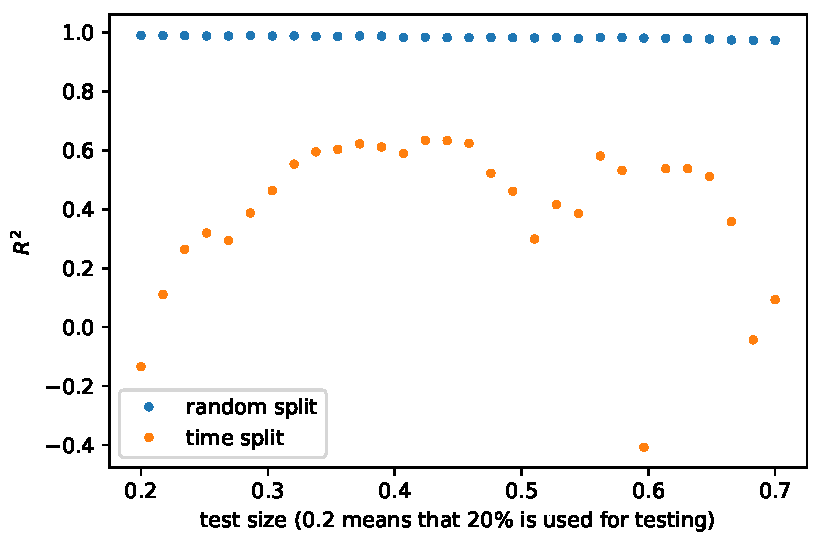
\includegraphics[width = 0.95\textwidth]{figures/test_size_variation.pdf}\end{center}
\vspace{-0.7cm}
\caption{Accuracy with a decision tree model for varying test sizes, using random test or rolling base test}
\label{fig:test_size_variation}
\end{figure}
\begin{figure}[H]
\begin{center}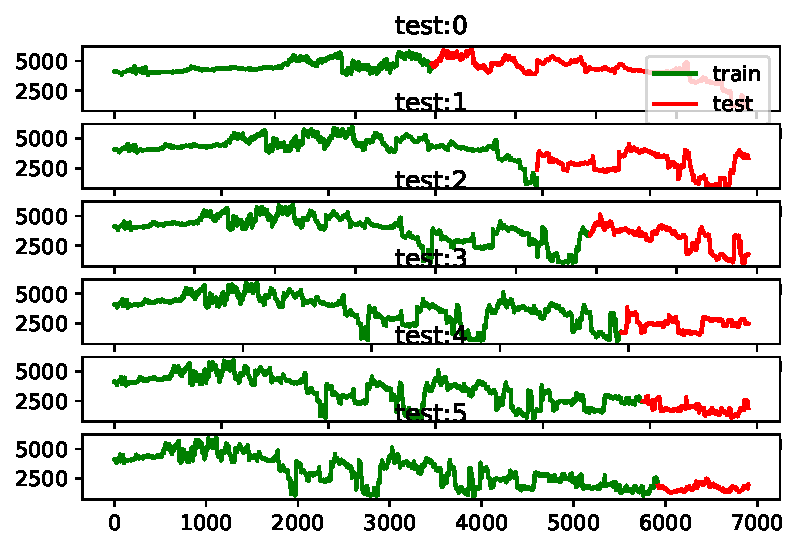
\includegraphics[width = 0.95\textwidth]{figures/rolling_basis.pdf}\end{center}
\vspace{-0.7cm}
\caption{Cross-validation on a rolling basis}
\label{fig:rolling_basis}
\end{figure}
